% Five points, no three collinear. Hull is a triangle; ABDE is a convex quadrilateral.
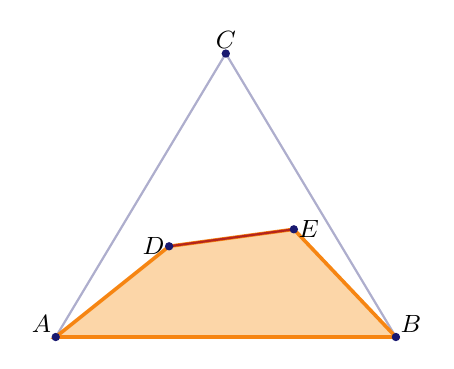
\begin{tikzpicture}[scale=0.72, every node/.style={font=\small}]
  \coordinate (A) at (0,0);
  \coordinate (B) at (6,0);
  \coordinate (C) at (3,5);
  \coordinate (D) at (2.0,1.6);
  \coordinate (E) at (4.2,1.9);
  \draw[MidnightBlue!35,thick] (A) -- (B) -- (C) -- cycle;
  \fill[BurntOrange!30] (A) -- (B) -- (E) -- (D) -- cycle;
  \draw[BurntOrange,line width=1.3pt] (A) -- (D) -- (E) -- (B) -- cycle;
  \draw[BrickRed,thick] (D) -- (E);
  \fill[MidnightBlue] (A) circle (2.1pt);
  \fill[MidnightBlue] (B) circle (2.1pt);
  \fill[MidnightBlue] (C) circle (2.1pt);
  \fill[MidnightBlue] (D) circle (2.1pt);
  \fill[MidnightBlue] (E) circle (2.1pt);
  \node[anchor=south east, inner sep=1.5pt] at (A) {$A$};
  \node[anchor=south west, inner sep=1.5pt] at (B) {$B$};
  \node[anchor=south, inner sep=1.5pt] at (C) {$C$};
  \node[anchor=east, inner sep=1.5pt] at (D) {$D$};
  \node[anchor=west, inner sep=1.5pt] at (E) {$E$};
\end{tikzpicture}
